% !TeX spellcheck = en_US
\addsection{Town}{\skills/artillery.png}

\begin{multicols*}{2}

\hypertarget{Town}{Each} Faction has their own Town, which is located in the center of their Starting Tile.
The Town is your most important location, as many scenarios \hyperlink{End}{may end} if it's \hyperlink{Categories}{Flagged} by an enemy Hero.\par
The contents of your Town and overall Faction status are represented by the Town Board.
It shows your currently built Buildings, Resource Costs for future Buildings, your Resource incomes and status of Town Action Tokens.\par
All Factions are able to Build the following Buildings in their Town:
\begin{itemize}
  \item \textbf{City Hall} – Provides Resource income or a Faction-Specific Ability.
  \item \textbf{Citadel} – Allows you to Reinforce units when using the Population Token.
Also \hyperlink{Walls}{protects your Town} when it is attacked.
  \item \textbf{Unit Dwellings} – Allows you to Recruit Units.
Dwellings have three Levels that unlock new Units, but which must be Built in the following order:\includesvg[height=10px]{\svgs/bronze.svg}\includesvg[height=10px]{\svgs/silver.svg}\includesvg[height=10px]{\svgs/golden.svg}
  \item \textbf{Mage guild} - gives you \hyperlink{spells}{Spells}.
  \item \textbf{Faction Building} - a Faction-Specific Building with a unique effect.
\end{itemize}
\textbf{A single Building} may be Built each round by using the Build Token.
When you build a Building, pay its cost in Resources, flip the Build Token to its inactive side, and place the new Building’s Cardboard Piece into its proper slot on the Town Board.
If the Building has any immediate effects upon Building it, resolve them now.\par
Built Buildings are always represented by a symbol within a circle.
Buildings that can be built in the future are represented by a rectangle that contains the Building's cost in Resources.
Many Building Tiles are double-sided, and may later be upgraded and flipped to represent two different buildings at the same time. Such upgrades must be Built in order.\par
If a Town or Settlement is attacked by an enemy hero and your Hero is not also on that Field, you may immediately \textbf{pay 8 gold} to fight a defending Combat \textbf{using only your Units}.
You cannot use your deck during that Combat as your Main Hero is not present.
Paying this gold represents the cost of transporting the army there.\par
When you \hyperlink{Categories}{Flag} a Town, take \hyperlink{End}{a Faction Cube} from its previous owner.

\vspace*{\fill}

\begin{center}
  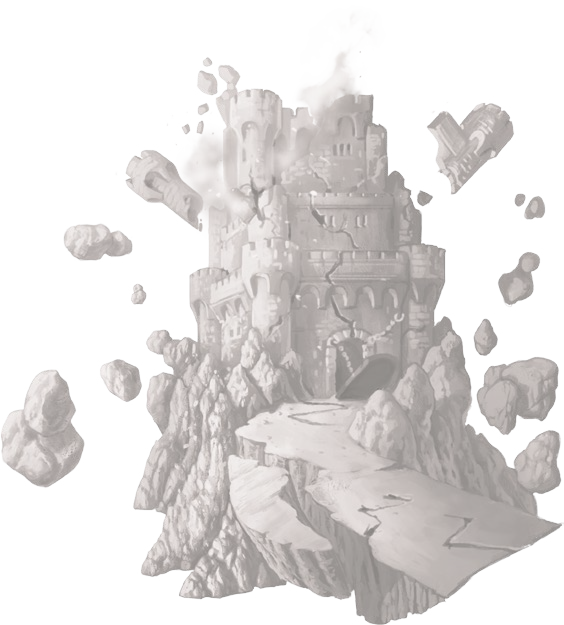
\includegraphics[width=\linewidth]{\art/earthquake.png}
\end{center}

\vspace*{\fill}

\end{multicols*}
